% latex uft-8
\documentclass[uplatex,a4paper,11pt,oneside,openany]{jsbook}
%
\usepackage[dvipdfmx]{graphicx}
\usepackage{amsmath,amssymb}
\usepackage{bm}
\usepackage{graphicx}
\usepackage{ascmac}
\usepackage{setspace}
\usepackage{here}
\usepackage{fancybox}
\usepackage{url}
\usepackage{comment}
\usepackage{listings,jlisting} %日本語のコメントアウトをする場合jlistingが必要
%ここからソースコードの表示に関する設定
\lstset{
  basicstyle={\ttfamily},
  identifierstyle={\small},
  commentstyle={\smallitshape},
  keywordstyle={\small\bfseries},
  ndkeywordstyle={\small},
  stringstyle={\small\ttfamily},
  frame={tb},
  breaklines=true,
  columns=[l]{fullflexible},
  numbers=left,
  xrightmargin=0zw,
  xleftmargin=3zw,
  numberstyle={\scriptsize},
  stepnumber=1,
  numbersep=1zw,
  lineskip=-0.5ex
}
%ここまでソースコードの表示に関する設定
\makeatletter
\def\ps@plainfoot{%
  \let\@mkboth\@gobbletwo
  \let\@oddhead\@empty
  \def\@oddfoot{\normalfont\hfil-- \thepage\ --\hfil}%
  \let\@evenhead\@empty
  \let\@evenfoot\@oddfoot}
  \let\ps@plain\ps@plainfoot
\renewcommand{\chapter}{%
  \if@openright\cleardoublepage\else\clearpage\fi
  \global\@topnum\z@
  \secdef\@chapter\@schapter}
\makeatother
%
\newcommand{\maru}[1]{{\ooalign{%
\hfil\hbox{$\bigcirc$}\hfil\crcr%
\hfil\hbox{#1}\hfil}}}
%
\setlength{\textwidth}{\fullwidth}
\setlength{\textheight}{40\baselineskip}
\addtolength{\textheight}{\topskip}
\setlength{\voffset}{-0.55in}
%
\begin{document}
% START DOCUMENT
%
% COVER
\begin{center}
  \huge \par
  \vspace{15mm}
  \huge 2020\par
  \vspace{15mm}
  \LARGE GPIO (Raspberry pi, Arduino)\par
  \vspace{100mm}
  \Large \date \par
  \vspace{15mm}
  \Large S.Matoike \par
  \vspace{10mm}
  \Large \par
  \vspace{10mm}
\end{center}
\thispagestyle{empty}
\clearpage
\addtocounter{page}{-1}
\newpage
\setcounter{tocdepth}{3}
%
\tableofcontents
%
\chapter{はじめに}
%
\chapter{GPIO}

\section{Raspberry pi}

\begin{minipage}{0.90\hsize}
      \centering
      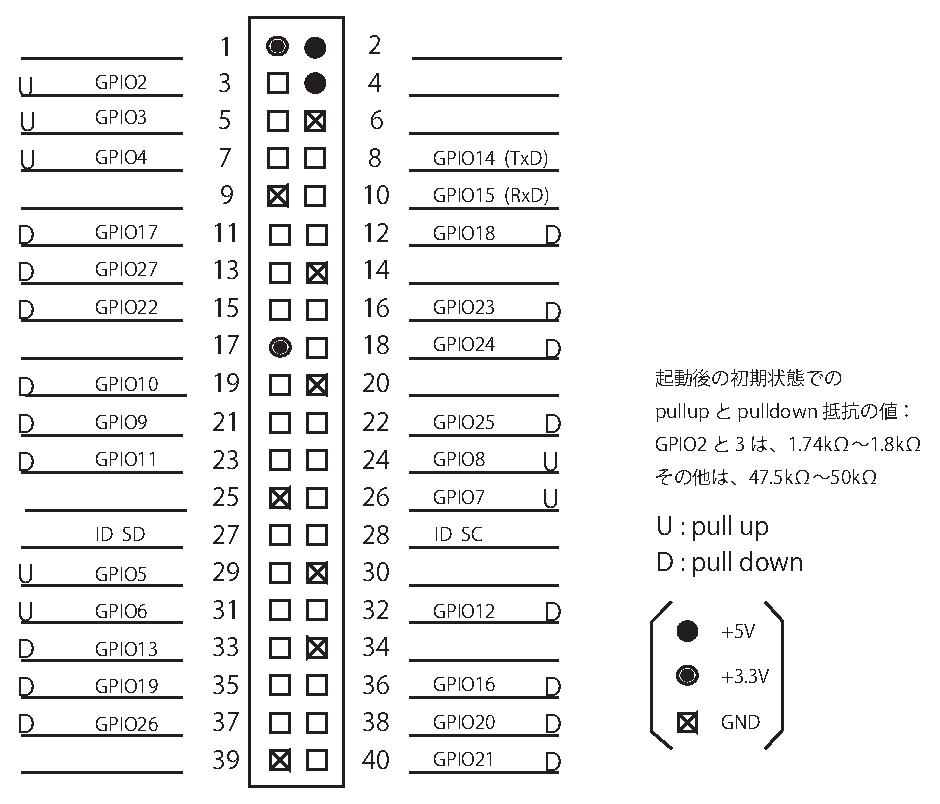
\includegraphics[keepaspectratio, scale=0.80, angle=0]
                      {figures/eps/raspiGPIO.eps}
                      %\caption{}
                      \label{fig:GPIO}
\end{minipage}

%\section{Arduino}

\chapter{デジタル入出力}

\section{LED(出力)}

%\subsection{Raspberry pi}

\begin{minipage}{0.90\hsize}
      \centering
      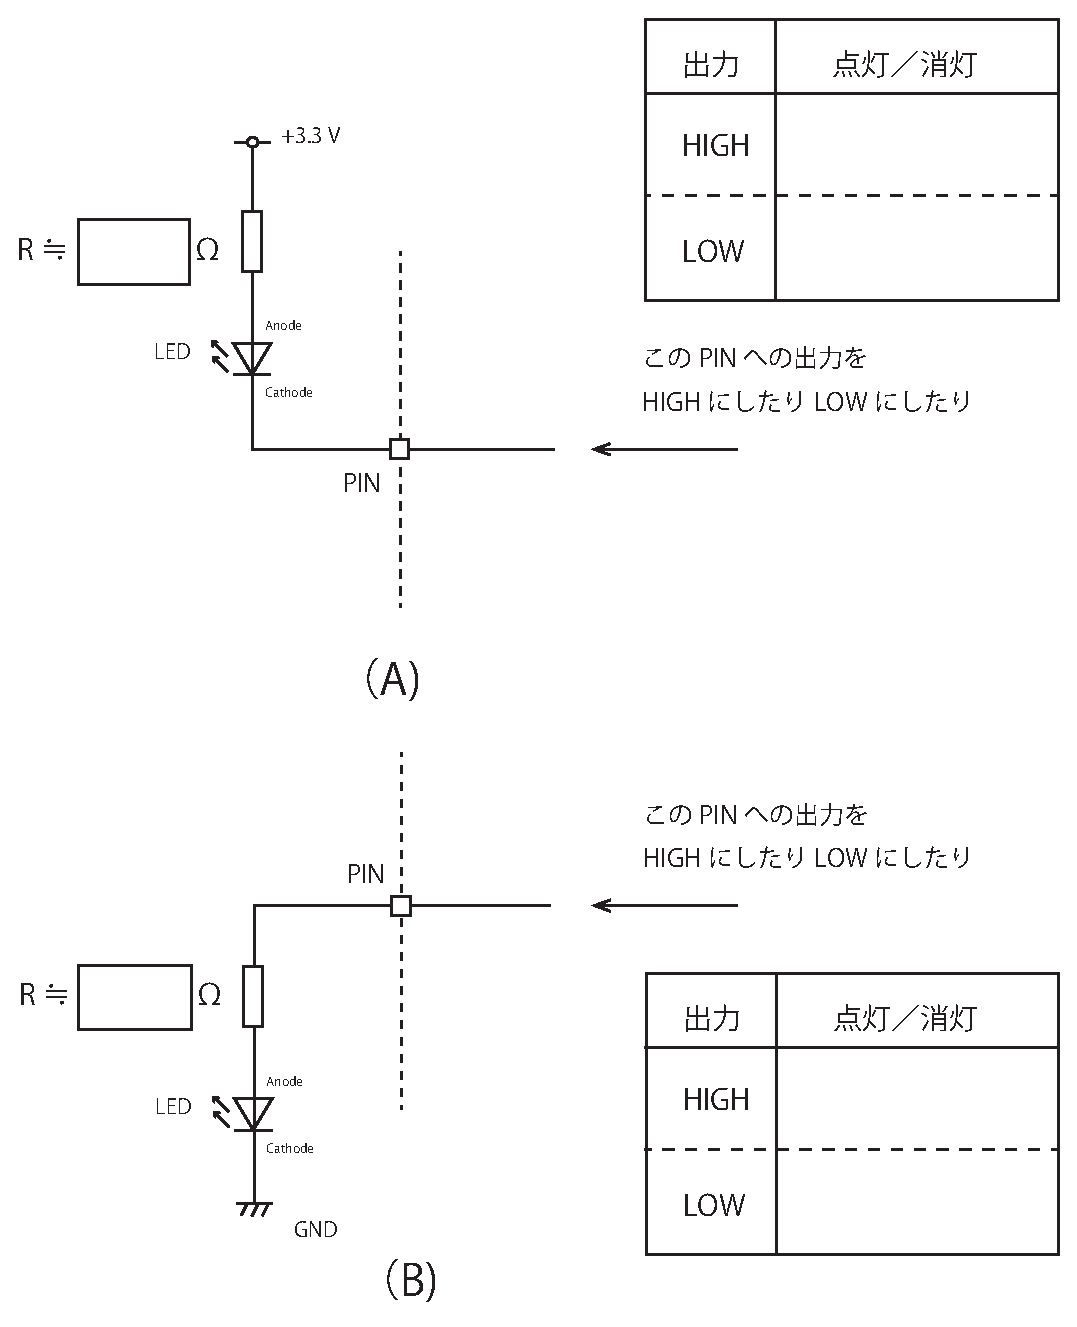
\includegraphics[keepaspectratio, scale=0.6, angle=0]
                      {figures/eps/led00alt.eps}
                      %\caption{}
                      \label{fig:LED}
\end{minipage}\\\\


※注意:GPIOの各ピンには、全てプルアップあるいはプロダウン抵抗が内蔵されているので、
外付けのLEDのための電流制限抵抗は無くても動作します\\

【演習1】次のことを確認してみよう(PIN番号は各自で任意に選択すること)

\begin{enumerate}
\item[(1)] 配布された外付け用の電流制限抵抗が何$\Omega$かテスターで調べてみよう
\item[(2)] Raspberry PiのPINで提供されている電源3.3VとGNDを、ブレッドボード上の赤と青のライン上に引き出し、実際の電圧をテスターで調べてみよう
\item[(3)] (A)の結線の場合には、GPIOのPINにHIGH(=1)を出力した時にLEDは消灯し、LOW(=0)を出力した時にLEDは点灯することをプログラムで確認しよう
\item[(4)] (B)の結線の場合には、GPIOのPINにHIGH(=1)を出力した時にLEDは点灯し、LOW(=0)を出力した時にLEDは消灯することをプログラムで確認しよう
\end{enumerate}

\begin{figure}[htpb]
  %\centering
    \begin{tabular}{lr}
      \begin{minipage}{0.55\hsize}
\begin{lstlisting}[caption=LED(C言語),label=prog2]
#include <stdio.h>
#include <wiringPi.h>
#define PIN 17
void main(void) {
   if( wiringPiSetupGpio() == -1) return;
   pinMode(PIN, OUTPUT);
   int a;
   do{
       printf("1 or 0 : ");
       scanf("%d", &a);
       if ( a==1 )
           digitalWrite(PIN, 1);
       else if ( a==0 )
           digitalWrite(PIN, 0);
       else
           break;
   } while( TRUE );
   digitalWrite(PIN, 0);
}
\end{lstlisting}
    \end{minipage}
    \begin{minipage}{0.5\hsize}
    \begin{lstlisting}[caption=LED(Python),label=prog1]
import RPi.GPIO as GPIO

PIN = 17
GPIO.setwarnings(False)
GPIO.setmode(GPIO.BCM)
GPIO.setup(PIN, GPIO.OUT)

while True:
    str = input('1 or 0 : ')
    a = int( str )
    if a==1:
        GPIO.output(PIN, GPIO.HIGH)
    elif a==0:
        GPIO.output(PIN, GPIO.LOW)
    else:
        break

GPIO.cleanup()
print('\n終わり!')
    \end{lstlisting}%
    \end{minipage}
  \end{tabular}
\end{figure}

C言語のプログラムでは、
ソースプログラムをled01.cという名称のテキストファイルとして保存し、
以下のようにgccコマンドでコンパイルして実行します

\begin{screen}
\$ \, gcc \, -o \, led01 \, led01.c \, -I/usr/local/include \, -L/usr/local/lib \, -$\ell$wiringPi\\
\$ \, ./led01
\end{screen}

物理的なピン配置の番号でPINを指定する場合には、

C言語では、wiringPiSetupGpio(void);に代えて、wiringPiSetupPhys(void);を使います。

Pythonでは、GPIO.setmode(GPIO.BCM)を、GPIO.setmode(GPIO.BOARD)に代えます。

【演習2】演習1のプログラムを、GPIO番号から物理的PIN配置番号に変更して動作を確認しよう

\subsection{シェル(コマンド)によるGPIOの操作}

wiringPiが使えるようになっているか否かを、次のようにバージョンを表示させて確認します

\begin{screen}
\$ \, gpio \, -v\\
gpio version: 2.50\\
Copyright (c) 2012-2018 Gordon Henderson\\
This is free software with ABSOLUTELY NO WARRANTY.\\
For details type: gpio -warranty\\
Raspberry Pi Details:\\
......
\end{screen}

wiringPiを使うと、プログラムを書かなくても、次のようにコマンドを打つだけでGPIOをON/OFFすることができます

\begin{screen}
\$ \, gpio \, -g \, mode \, 17 \, out\\
\$ \, gpio \, -g \, write \, 17 \, 1\\
\$ \, gpio \, -g \, write \, 17 \, 0
\end{screen}

$-g$という指定は、ピン番号にGPIOのピン番号を使う場合に指定します(この例ではGPIO17)

この指定をしなかった場合のデフォルトは、物理的な配置番号(コネクタの番号)になります

bashのシェルスクリプトにまとめるとすると、次のように書くことができます

\begin{lstlisting}[caption=LED(shell),label=prog1]
#!/bin/bash
set -euo pipefail
LED_PIN = 23
gpio export $LED_PIN out
trap 'gpio unexport $LED_PIN' SIGINT
while true
do
   gpio -g write $LED_PIN 1
   sleep 1
   gpio -g write $LED_PIN 0
   sleep 1
done
\end{lstlisting}

これを、led01.sh という名前のテキストファイルに保存し、chmodコマンドを使ってファイルに実行権限を与え、その上で実行します

「ls \, -l」として、ファイルの属性を表示させてみると、実行権限が与えられたことを確認できます

ファイルに実行権限を与えない場合でも、「sh \, ./led01.sh」 としてシェルを実行させることも可能です

\begin{screen}
\$ \, chmod \, +x \, ./led01.sh\\
\$ \, ./led01.sh
\end{screen}

(参考:bashのオプション)
\begin{enumerate}
\item[set -e:] 実行されたコマンドの1つが0でないステータスで終了した場合、スクリプトを終了させ、エラーシェルスクリプト実行時に実行内容が表示させるようにするオプション
\item[set -u:] 未定義変数が参照されたときに処理を終了します(ーの代わりに+を指定すると意味は逆になります)
\item[set -o:] 続けてpipefailを指定します。パイプでつないだ各コマンドの中で、終了ステータスが0(正常終了)以外だった場合に、最後に0以外だったコマンドの終了ステータスが返されます
\item[set -n:] スクリプト自体は実行されず、文法チェックのみが行われる(問題なければ何も出力されません)
\item[set -v:] シェルスクリプト内でこれから実行されるコマンドを表示します。これは、スクリプト内に記述されているコマンドが出力されるだけなので、実際の使用に当たっては、「-x」オプションと一緒に指定して、実行する内容と、実行された内容を表示させるようにして使います
\item[set -x:] デバッグ情報の出力指示です。シェルスプリプと実行の際に、変数への代入や実行されたコマンドなど、シェルスクリプト内で処理された内容が表示されます
\end{enumerate}

%\subsection{Arduino}

\section{(Limit)Switch(入力)}

\begin{minipage}{0.90\hsize}
      \centering
      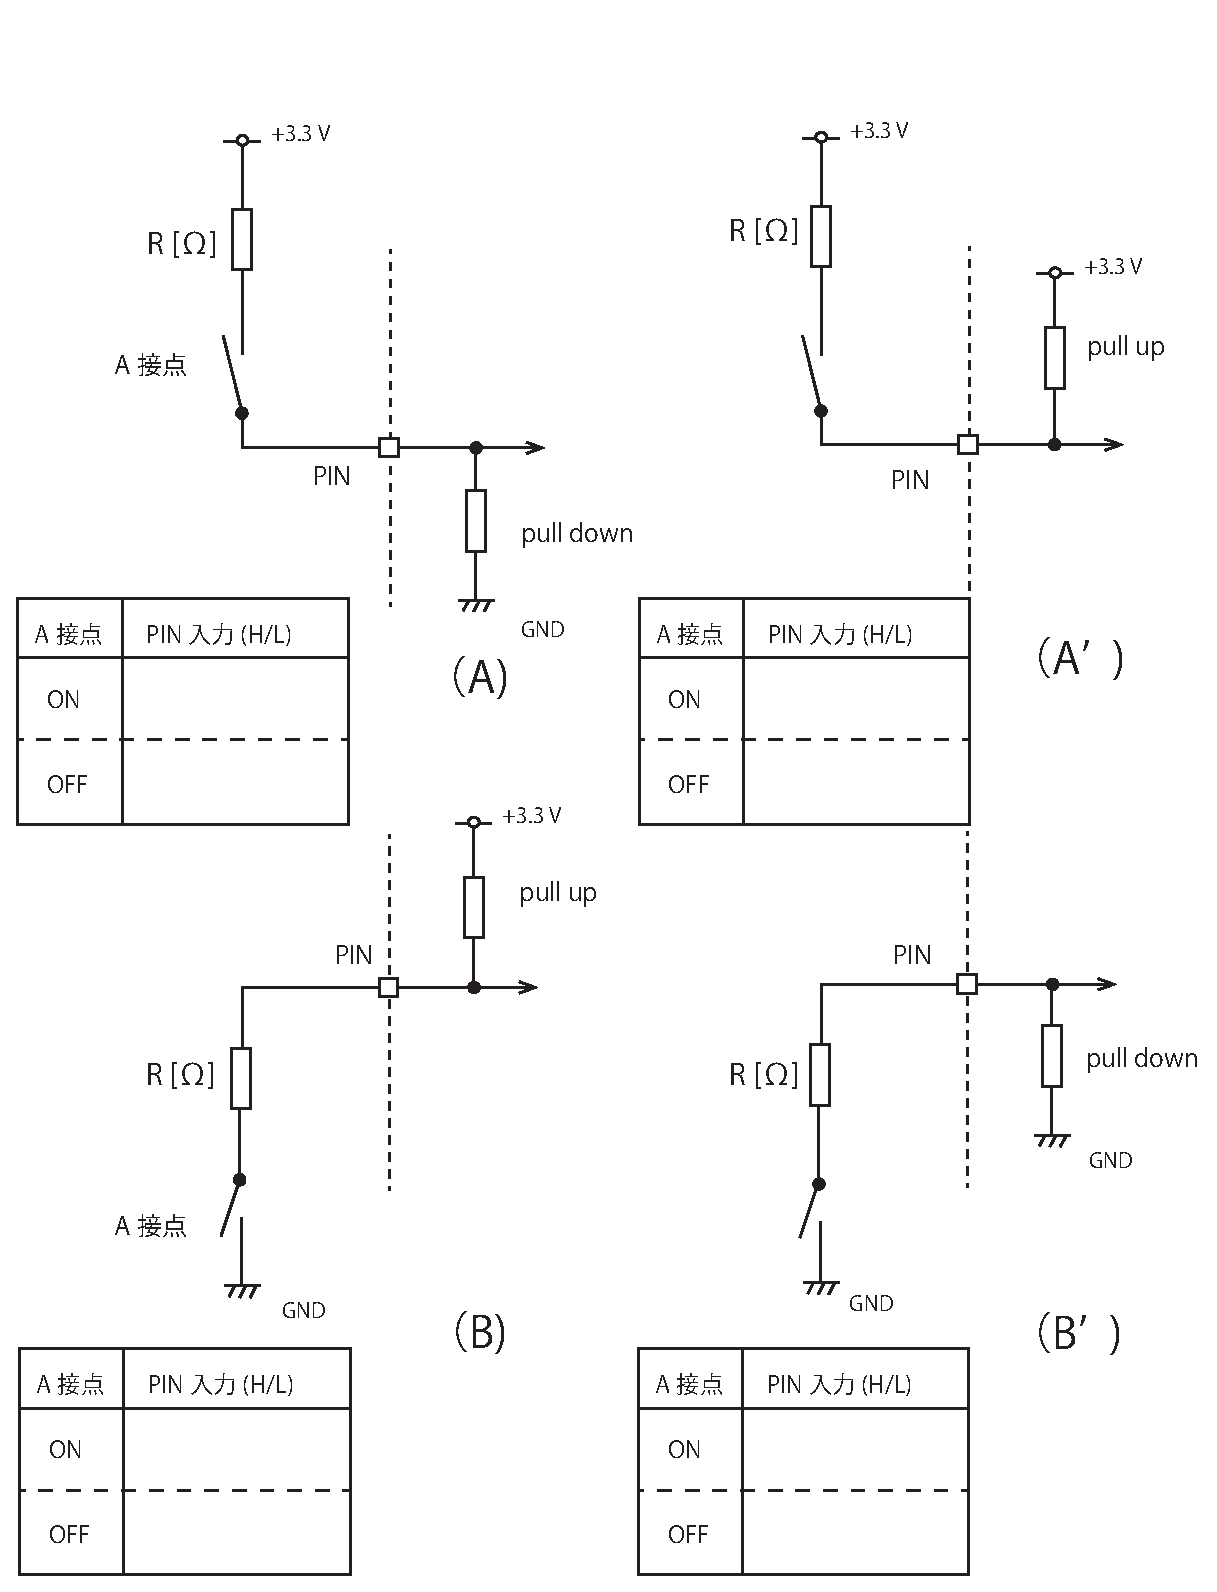
\includegraphics[keepaspectratio, scale=0.6, angle=0]
                      {figures/eps/switch00.eps}
                      %\caption{}
                      \label{fig:LED}
\end{minipage}\\

※注意:GPIOの各ピンには、全てプルアップあるいはプロダウン抵抗が内蔵されているので、
外付けの抵抗R[$\Omega$]は無くても動作します\\

GPIOのPINを入力(INPUT)のモードで使うときには、プルアップ(PUD\_UP)あるいはプルダウン(PUD\_DOWN)を指定して、
PINの初期状態を切り替えることができます(なおGPIOのPINを出力(OUTPUT)のモードで使うときには、この指定はできません)

%GPIO2とGPIO3の場合、他のGPIO端子の場合よりもプルアップあるいはプルダウンのための抵抗の値が小さいので、

(A')の結線では、Switchの状態とは無関係に、PINの状態がLOW(=0)になることはありません

(B')の結線では、Switchの状態とは無関係に、PINの状態がHIGH(=1)になることはありません

つまり、(A')や(B')の結線ではSwitchの状態を読むことはできません(このような使い方は無い)

【演習3】次のことを確認してみよう(PIN番号は各自で任意に選択すること)

\begin{enumerate}
\item[(1)] 配布したLimit Switchには端子が3本あります。A接点とB接点が内蔵されているのですが、
どの端子とどの端子を使えばA接点になるのか、どの端子とどの端子を使えばB接点になるのか、テスターで調べてみましょう
\item[(2)] (A)の結線の様にPINをプルダウンしている場合、A接点がONならPINの入力はHIGH(=1)に、
A接点がOFFならPINの入力はLOW(=0)になることをプログラムで確認しよう
\item[(3)] (B)の結線の様にPINをプルアップしている場合、A接点がONならPINの入力はLOW(=0)に、
A接点がOFFならPINの入力はHIGH(=1)になることをプログラムで確認しよう
\item[(4)](A')や(B')の結線ではSwitchの状態を読みとれないことを、プログラムで確認しましょう\\
\end{enumerate}

\begin{figure}[htpb]
  %\centering
    \begin{tabular}{lr}
      \begin{minipage}{0.5\hsize}
\begin{lstlisting}[caption=Switch(C言語),label=prog2]
#include <stdio.h>
#include <wiringPi.h>

#define PIN 27

void main(void) {
   if( wiringPiSetupGpio() == -1) return;
   pinMode(PIN, INPUT);
   pullUpDnControl(PIN, PUD_UP);

   do{
      int a = digitalRead(PIN);
      if ( a==1 )
         printf("%d:Switch ON\n", a);
      else
         printf("%d:Switch OFF\n", a);
      delay(1000);
   } while( TRUE );
}
\end{lstlisting}
    \end{minipage}

    \begin{minipage}{0.5\hsize}
    \begin{lstlisting}[caption=Switch(Python),label=prog4]
import RPi.GPIO as GPIO
from time import sleep

PIN = 27
GPIO.setwarnings(False)
GPIO.setmode(GPIO.BCM)
GPIO.setup(PIN, GPIO.IN,\
           pull_up_down=GPIO.PUD_UP)
try:
  while True:
    a = GPIO.input(PIN)
    if a==1:
       print( str(a) + ':Switch ON' )
    else:
       print( str(a) + ':Switch OFF' )
    sleep(1.0)
except KeyboardInterrupt:
    pass
finally:
    GPIO.cleanup()
    \end{lstlisting}%
    \end{minipage}
  \end{tabular}
\end{figure}%

wiringPiを使うと、特別なプログラムを書かずに、次のようにコマンドを並べるだけでGPIOからPINの値を読み取ることができます

\begin{screen}
\$ \, gpio \, -g \, mode \, 3 \, in\\
\$ \, gpio \, -g \, read \, 3
\end{screen}

bashのシェルスクリプトにこれらのコマンドをまとめると、
次のようにしてプログラムを書いた場合と同じようにしてシェルスクリプトを使うことができます\\

\begin{lstlisting}[caption=SW(shell),label=prog1]
#!/bin/bash
set -euo pipefail
SW_PIN = 3
gpio export $SW_PIN in
trap 'gpio unexport $SW_PIN' SIGINT
while true
do
   gpio -g read $SW_PIN
   sleep 1
done
\end{lstlisting}

【演習4】プログラムを作成して確認しましょう(各PINのGPIO番号は任意に選択すること)

\begin{enumerate}
\item[(1)] (A)の結線のA接点がONの時はLEDが点灯し、OFFの時は消灯するプログラム
\item[(2)] (B)の結線のA接点がONの時はLEDが点灯し、OFFの時は消灯するプログラム
\end{enumerate}

\begin{minipage}{0.90\hsize}
      \centering
      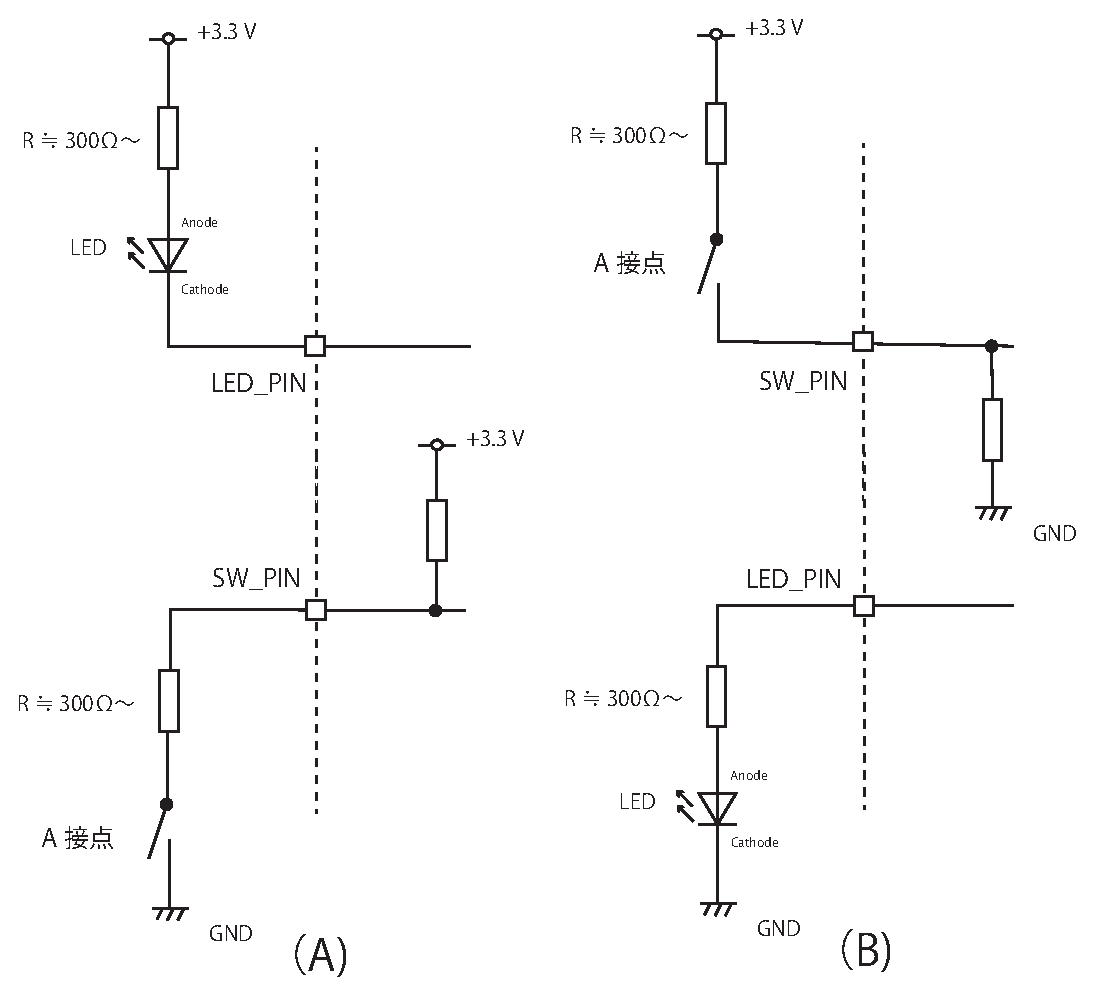
\includegraphics[keepaspectratio, scale=0.7, angle=0]
                      {figures/eps/ledsw.eps}
                      %\caption{}
                      \label{fig:LED}
\end{minipage}

\newpage

\section{Photo interrupter, reflector(入力)}

フォトインタラプタは、光を遮光する箇所をリミットスイッチとして使ったり、遮光した回数を数えたりする場面で利用されます

フォトリフレクタは、物体に当てた光の反射を受信検知するもので、物体の通過を知るときなどに使われます。
プログラム上での扱い方は、フォトリフレクタやインタラプタ、その他のスイッチでも同じです

\begin{minipage}{0.90\hsize}
      \centering
      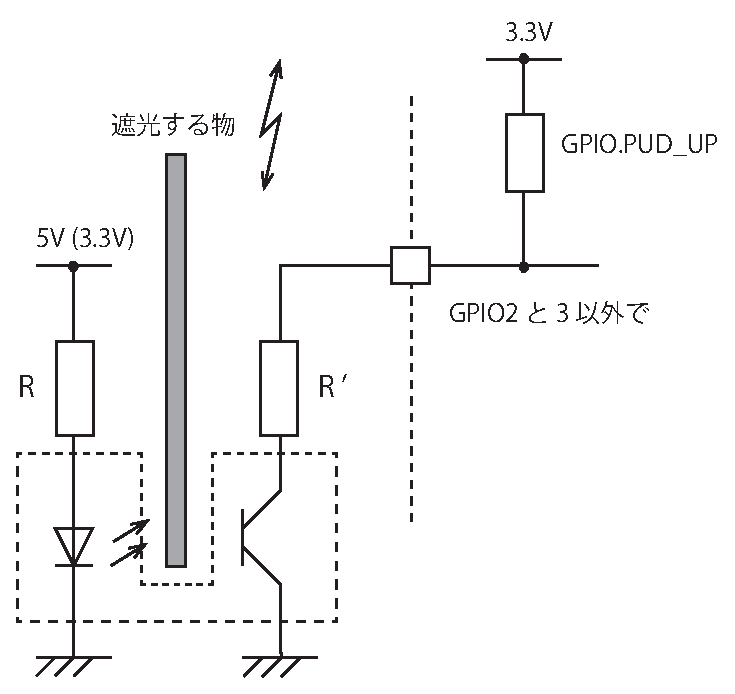
\includegraphics[keepaspectratio, scale=0.5, angle=0]
                      {figures/eps/PhotoInterrupter.eps}
                      %\caption{}
                      \label{fig:PI}
\end{minipage}\\

注意:抵抗器 R' は、プルアップ抵抗が内蔵されているので必ずしも必要ではありません

動作確認のプログラムはスイッチの時と同様に記述できますが、Arduino風に書くことに倣うと次のように書くことができます。
setup()関数とloop()関数を中心に記述していくことができます

\begin{lstlisting}[caption=Photo interrupter(Python),label=prog2]
import RPi.GPIO as GPIO
import time
PIPin = 4
def setup():
    GPIO.setwarnings( False )
    GPIO.setmode( GPIO.BCM )
    GPIO.setup( PIPin, GPIO_IN, pull_up_down=GPIO.PUD_UP )

def loop():
    v = GPIO.input( PIPin )
    print( v )
    time.sleep( 1.0 )

if __name__ == '__main__':
    setup()
    try:
        while True:
            loop()
    except KeyboardInterrupt:
        pass
    finally:
        GPIO.cleanup()
\end{lstlisting}%

【演習5】上記プログラムを以下の課題に対応させるように書き換えてみましょう
\begin{enumerate}
\item[(1)] 演習4の回路(A)のスイッチをフォトインタラプタに代えて、遮光時にLEDを点灯させる動作
\item[(2)] 遮光した回数をカウントし、その回数が5の倍数の時にLEDを5秒間点灯させる動作
\item[(3)] C言語でも動作を確認してみましょう
\end{enumerate}

\section{3.3Vと5Vの世界の橋渡し}

\subsection{Photo coupler(出力・入力)}

\subsection{CMOSとTTL}

\subsection{Interrupt(割り込み)}

\begin{figure}[htpb]
  %\centering
    \begin{tabular}{lr}
      \begin{minipage}{\hsize}

\begin{lstlisting}[caption=Interrupt(Python),label=prog2]
import RPi.GPIO as GPIO

PIN1 = 23
PIN2 = 24
GPIO.setwarnings(False)
GPIO.setmode(GPIO.BCM)
GPIO.setup(PIN1, GPIO.IN, pull_up_down=GPIO.PUD_UP)
GPIO.setup(PIN2, GPIO.IN, pull_up_down=GPIO.PUD_DOWN)

def myCallback(channel):
    print(str(PIN1) + ' was pushed:' + str(channel))

GPIO.add_event_detect(PIN2, GPIO.RISING, callback=myCallback, bouncetime=300)

try:
    print('waiting for falling edge on port ' + str(PIN1))
    GPIO.wait_for_edge(PIN1, GPIO.FALLING)    # FALLING, RISING, BOTH
    print(str(PIN1) + ' was pressed')
except KeyboardInterrupt:
    pass
finally:
    GPIO.cleanup()
\end{lstlisting}

    \end{minipage}
    \begin{minipage}{0\hsize}
    %\begin{lstlisting}[caption=Interrupt2(Python),label=prog4]

    %\end{lstlisting}%
    \end{minipage}
  \end{tabular}
\end{figure}%

【演習6】演習4の課題を使って、次のことを試してしてみましょう

\begin{enumerate}
\item[(1)] 演習4の課題そのままを、割り込みを使って実現する処理
\item[(2)] (A)又は(B)の結線で、A接点をON(直後にOFF)にした時にLEDが点灯し、再度ON(直後にOFF)とした時に消灯する処理
\end{enumerate}

\subsection{チャタリング対策}

\begin{comment}

\section{Rotary Encoder(入力)}

\url{https://www.sunfounder.com/}

\begin{lstlisting}[caption=Rotary Encoder(C言語),label=prog2]
#include <stdio.h>
#include <string.h>
#include <errno.h>
#include <stdlib.h>
#include <wiringPi.h>

#define  RoAPin    0
#define  RoBPin    1
#define  RoSPin    2

static volatile int globalCounter = 0;

unsigned char flag;
unsigned char Last_RoB_Status;
unsigned char Current_RoB_Status;

void rotaryDeal(void){
  Last_RoB_Status = digitalRead(RoBPin);

  while(!digitalRead(RoAPin)){
    Current_RoB_Status = digitalRead(RoBPin);
    flag = 1;
  }

  if(flag == 1){
    flag = 0;
    if((Last_RoB_Status == 0)&&(Current_RoB_Status == 1)){
      globalCounter ++;
      printf("globalCounter : %d\n",globalCounter);
    }
    if((Last_RoB_Status == 1)&&(Current_RoB_Status == 0)){
      globalCounter --;
      printf("globalCounter : %d\n",globalCounter);
    }

  }
}

void rotaryClear(void){
  if(digitalRead(RoSPin) == 0){
    globalCounter = 0;
    printf("globalCounter : %d\n",globalCounter);
    delay(1000);
  }
}

int main(void){
  if(wiringPiSetup() < 0){
    fprintf(stderr, "Unable to setup wiringPi:%s\n",strerror(errno));
    return 1;
  }

  pinMode(RoAPin, INPUT);
  pinMode(RoBPin, INPUT);
  pinMode(RoSPin, INPUT);

  pullUpDnControl(RoSPin, PUD_UP);

  while(1){
    rotaryDeal();
    rotaryClear();
  }

  return 0;
}
\end{lstlisting}



\begin{lstlisting}[caption=Rotary Encoder(Python),label=prog4]
import RPi.GPIO as GPIO
import time

RoAPin = 11    # pin11
RoBPin = 12    # pin12
RoSPin = 13    # pin13

globalCounter = 0

flag = 0
Last_RoB_Status = 0
Current_RoB_Status = 0

def setup():
  GPIO.setmode(GPIO.BOARD)       # Numbers GPIOs by physical location
  GPIO.setup(RoAPin, GPIO.IN)
  GPIO.setup(RoBPin, GPIO.IN)
  GPIO.setup(RoSPin, GPIO.IN, pull_up_down=GPIO.PUD_UP)
  rotaryClear()

def rotaryDeal():
  global flag
  global Last_RoB_Status
  global Current_RoB_Status
  global globalCounter
  Last_RoB_Status = GPIO.input(RoBPin)
  while(not GPIO.input(RoAPin)):
    Current_RoB_Status = GPIO.input(RoBPin)
    flag = 1
  if flag == 1:
    flag = 0
    if (Last_RoB_Status == 0) and (Current_RoB_Status == 1):
      globalCounter = globalCounter + 1
      print 'globalCounter = %d' % globalCounter
    if (Last_RoB_Status == 1) and (Current_RoB_Status == 0):
      globalCounter = globalCounter - 1
      print 'globalCounter = %d' % globalCounter

def clear(ev=None):
  globalCounter = 0
  print 'globalCounter = %d' % globalCounter
  time.sleep(1)

def rotaryClear():
  GPIO.add_event_detect(RoSPin, GPIO.FALLING, callback=clear) # wait for falling


def loop():
  global globalCounter
  while True:
    rotaryDeal()
#   print 'globalCounter = %d' % globalCounter

def destroy():
  GPIO.cleanup() # Release resource

if __name__ == '__main__':
  setup()
  try:
    loop()
  except KeyboardInterrupt:
    destroy()
\end{lstlisting}%


\begin{lstlisting}[caption=Alternate Rotary Encoder(Python),label=prog4]
#http://www.ozeki.hu/p_3054-how-to-setup-a-rotary-encoder-on-raspberry-pi.html
import RPi.GPIO as GPIO
from time import sleep

counter = 10
Enc_A = 17
Enc_B = 27

def init():
    print "Rotary Encoder Test Program"
    GPIO.setwarnings(True)
    GPIO.setmode(GPIO.BCM)
    GPIO.setup(Enc_A, GPIO.IN)
    GPIO.setup(Enc_B, GPIO.IN)
    GPIO.add_event_detect(Enc_A, GPIO.RISING, callback=rotation_decode, bouncetime=10)
    return

def rotation_decode(Enc_A):
    global counter
    sleep(0.002)
    Switch_A = GPIO.input(Enc_A)
    Switch_B = GPIO.input(Enc_B)

    if (Switch_A == 1) and (Switch_B == 0):
        counter += 1
        print "direction -> ", counter
        while Switch_B == 0:
            Switch_B = GPIO.input(Enc_B)
        while Switch_B == 1:
            Switch_B = GPIO.input(Enc_B)
        return

    elif (Switch_A == 1) and (Switch_B == 1):
        counter -= 1
        print "direction <- ", counter
        while Switch_A == 1:
            Switch_A = GPIO.input(Enc_A)
        return
    else:
        return

def main():
    try:
        init()
        while True :
            sleep(1)

    except KeyboardInterrupt:
        GPIO.cleanup()

if __name__ == '__main__':
    main()
\end{lstlisting}%

\url{http://www.ozeki.hu/p_3054-how-to-setup-a-rotary-encoder-on-raspberry-pi.html}

Raspberry PI Rotary Encoder Control Code

Rotary encoders are designed for infinite circular turns in both direction. You can press the top button to send out an extra event. Encoders can sense if they are turned in full, half or quarter rounds depending on the type of the encoder. They send out these turns in bit arrays. To see the prompt bit arrays you should receive, please check the datasheet of the encoder you are using. You can find datasheets on the internet. When the rotary encoder is turned by someone or the button is pressed an event is sent from the device.

Required hardware
Raspberry PI
Rotary encoder
3 Resistors 1kΩ
Source code to install on controller

\begin{lstlisting}[caption=Alternate Rotary Encoder(Python),label=prog4]
import RPi.GPIO as GPIO
from time import sleep

counter = 10

Enc_A = 17
Enc_B = 27

def init():
    print "Rotary Encoder Test Program"
    GPIO.setwarnings(True)
    GPIO.setmode(GPIO.BCM)
    GPIO.setup(Enc_A, GPIO.IN)
    GPIO.setup(Enc_B, GPIO.IN)
    GPIO.add_event_detect(Enc_A, GPIO.RISING, callback=rotation_decode, bouncetime=10)
    return

def rotation_decode(Enc_A):
    global counter
    sleep(0.002)
    Switch_A = GPIO.input(Enc_A)
    Switch_B = GPIO.input(Enc_B)

    if (Switch_A == 1) and (Switch_B == 0):
        counter += 1
        print "direction -> ", counter
        while Switch_B == 0:
            Switch_B = GPIO.input(Enc_B)
        while Switch_B == 1:
            Switch_B = GPIO.input(Enc_B)
        return

    elif (Switch_A == 1) and (Switch_B == 1):
        counter -= 1
        print "direction <- ", counter
        while Switch_A == 1:
            Switch_A = GPIO.input(Enc_A)
        return
    else:
        return

def main():
    try:
        init()
        while True :
            sleep(1)

    except KeyboardInterrupt:
        GPIO.cleanup()

if __name__ == '__main__':
    main()
\end{lstlisting}%

%\subsection{Raspberry pi}

%\subsection{Arduino}

\section{Relay(出力)}

\subsection{機械接点}

\subsection{Solid State Relay(SSR)}

\subsection{ソレノイド}

\section{Servo Motor(出力)}

\url{https://www.learnrobotics.org/blog/raspberry-pi-servo-motor/}

How to Control a Servo with Raspberry Pi
07/16/2020
We sometimes use affiliate links in our content. This won't cost you anything, but it helps us to offset the costs of paying our writing team. You can support us directly on BuyMeACoffee. Thank you!

Are you looking to interface Raspberry Pi with a servo motor? Are you confused about how servo motors work?

Well, you’ve come to the right place! In this article, I will show you how to wire and program servo motors using Python and demystify the concept of the “duty cycle” to calculate the servo angle.

Ready to get started?

Table of Contents

サーボモータ対DCモータ

サーボモータって何?サーボモータは、指定した角度だけ回転できるDCモータの一種です。DCモータは磁力を使って電気的エネルギを機械的エネルギに変換するモータです。
サーボモータとDCモータの違いは、サーボモータが回転角度を制御できるのに対して、DCモータはただON/OFFを制御できるだけだという点にあります。

Servo Motor vs. DC Motor

What is a servo motor? A servo motor is a type of DC motor that can rotate to a specified angle. A DC Motor is a type of motor that converts electrical energy into mechanical energy using a magnetic force. The difference between a servo motor vs. a DC motor is that you can control the angle of a servo motor whereas with a DC motor you can only control whether the motor is on or off.

servo motors vs dc motors

もしDCモータで、速度、方向、そして位置を制御したいなら、モータコントローラやエンコーダを用意する必要があるでしょう(L298Nをおすすめします)。サーバモータの最も大きな優位性は、角度を制御できることです。そしてそれは、DCモータのように追加のセンサを必要とせずに、度のレベルの精度で達成できるのです。

If you want to control the speed, direction, and position of a DC motor, you’ll need to use a motor controller and an encoder, respectively. (I recommend the L298N.) The biggest advantage of servo motors is that you can precisely control the angle of the servo. Unlike DC motors, you won’t need any additional sensors to achieve degree-level precision and accuracy.

サーボモータのもう一つの優位性は、コントローラを必要としないことです。主要なコントローラ(Raspberry Pi や Arduino)上のピンに、中間に素子を使うこと無く、直接サーバモータを接続できるのです。このことは、結線と設定を容易にすることになります。

Another advantage of using servo motors is that you don’t need a motor controller. You can connect a servo motor directly to the pins on the majority of controllers (Raspberry Pi and Arduino) without using an intermediary chip. This makes wiring and configuration super easy.

サーボモータの種類
Types of Servo Motors

多くのサーボモータは連続していない。つまり、360度フルに回転できません。大部分のサーボモータは、0−180度の範囲で動作します。
あなたのサーボモータの、最小位置と最大位置を決めているデータシートを確認してみましょう。3種類のサーボモータがよく使われます。
それは、9gサーボモータ、MG99Rサーボモータ、そして連続回転サーボモータです。

Most servo motors are not continuous. That means they cannot rotate a full 360 degrees. Most servo motors have a range of 0-180 degrees. Check the datasheet for your servo to determine its minimum and maximum positions. Three types of Servo motors that are popular are the 9g Servo Motor, the MG996R Servo Motor, and the Continuous Rotation Servo Motor.

servo motors hobby project

9gサーボモータ
9g Servo Motor

あなたがロボット工学や趣味のプロジェクトに関わっているなら、SG90 9gサーボモータの選択は人気がある。
SG90は小さくて軽く出力の大きいサーボモータです。それは180度(+-両方向に90度)回転します。伝統的なサーボモータ同様、3本の線(GND、信号、電源)を持っています。
If you’re into robotics or hobby projects, the SG90 9g Servo motor (datasheet) is a popular choice. The SG90 is a small and lightweight servo motor with high output power. It can rotate 180 degrees (90 in either direction). Like traditional servo motors, this motor has three wires (ground, signal, and power).

MG996Rサーボモータ
MG996R Servo Motor

もう一つの人気のあるサーボモータは、MG996R高トルクデジタルサーボです。
それは、120度(+-両方向に60度)回転します。
SG90とMG996Rの両方とも、似たようなデューティ比とPWN周期を持っています。
PWMと回転角度の図を示します。

Another popular servo motor is the MG996R high-torque digital servo. It can rotate 120 degrees (60 in either direction). Both the SG90 and the MG996R have a similar Duty Cycle and PWM period. I’ve included the PWM diagram and angular rotation charts, below.

Raspberry PiのPWMによるサーボ制御
control servo with PWM Raspberry Pi

デューティー比の周期、あるいはデューティー比の周期を角度(度)に変換したものを使って、サーボを制御できます
You can control the servo by providing a duty cycle (\%) or converting the duty cycle to an angle measurement (in degrees).
Click here to view the calculations.

連続回転サーボ
Continuous Rotation Servo

連続的に回転するサーボ(FT90Rサーボのように)は、360度回転します
A continuous rotation servo (like the FT90R servo) rotates 360 degrees.
これは、モーターコントローラ無しでロボットを作ろうとしたら、あるいは360度を超える回転の高い精度を必要とするなら、これは大きな選択肢になります
This is a great option if you want to build a mobile robot without using a motor controller or if you need high precision over 360 degrees of rotation.
大部分の趣味のサーボにおいて一つ注意しておくことは、サーボの停止や逆転はそれを傷めることになります
One thing to note is that as with most hobby servos, stalling or back-driving servos can damage it.

ロボットにおける連続回転サーボ
continuous rotation servos for robotics
Raspberry PiのPWMを使ったサーボモータ制御
Servo Motor Control using PWM with Raspberry Pi
サーボは、Raspberry PiからのPWM(Pulse-Width Modulation)信号を使って制御されます
Servos are controlled using a Pulse-Width Modulation (PWM) signal from the Raspberry Pi.
PWMは、アナログ風の装置を制御することを許すデジタル信号の一つです
PWM is a type of digital signal that allows us to control devices in an analog fashion.
PWMは、信号がHIGHあるいはLOWの時間の大きさを変化させます
PWM varies the amount of time a signal is HIGH or LOW.
結果として、サーボモータの角度を制御に使われる信号の変化が得られる
As a result, we get a variable signal that can be used to control the angle of a Servo motor.

In this section, you’ll learn how to calculate the duty cycle for your servo motor using the datasheet. We’ll use the popular SG90 9g servo as an example; however, this methodology can be used for the majority of off-the-shelf servo motors.

CanaKit Raspberry Pi 4 4GB Starter Kit - 4GB RAM
Includes Raspberry Pi 4 4GB Model B with 1.5GHz 64-bit quad-core CPU (4GB RAM); 32GB Samsung EVO+ Micro SD Card (Class 10) Pre-loaded with NOOBS, USB MicroSD Card Reader

Step 1. Connect the Servo Motor to the Raspberry Pi using the Wiring Diagram

Here’s a Servo Motor Wiring Diagram for Arduino. All you need is a Raspberry Pi, 3 jumper wires, and a Servo Motor. You can also purchase a kit that has all of these components. Servo motors have three wires (ground, signal, and power). First, attach the ground wire to GND on the Raspberry Pi. Next, connect the signal wire to a GPIO pin on the Raspberry Pi. Finally, attach the power pin to 5V on the Raspberry Pi.

connect a servo to Raspberry Pi wiring diagram fritzing

Once you have the servo motor wired to the Raspberry Pi, it’s time to run some tests to verify servo positions.

Step 2. Verify servo motor positions using the Raspberry Pi Example Code

First, grab a copy of the servo’s datasheet. Then, look for the PWM diagram. You want to find the duty cycle range and/or the “neutral” position pulse duration.

how to read SG90 servo datasheet

Once you have those, I recommend creating a three-position chart for left, neutral (center), and right. Annotate your diagram with the angle (degrees) and Duty Cycle (ms) for each of the three positions. See the chart below.

control servo with PWM Raspberry Pi

Next, convert the duty cycle times to percentages by dividing the position’s duty cycle by the total PWM Period (20 ms). For example, the left position has a duty cycle = 1 ms. Therefore, 1/20 x 100% = 5%. I’ve included this handy chart for your reference.

Left	Neutral	Right
Angle (deg)	-90	0	+90
Duty Cycle (ms)	1 ms	1.5 ms	2 ms
Duty Cycle (%)	5%	7.5%	10%
Now that you have the duty cycle percentages for the three positions, it’s time to verify that these percentages accurately represent each of these positions. We’ll do this by using the RPi.GPIO library and writing Python code on the Raspberry Pi.

First, import the RPi.GPIO library and the sleep function.

import RPi.GPIO as GPIO
from time import sleep
Then, setup the GPIO mode as BOARD so that you can reference the PINs and not the BCM pins. (Feel free to use the BCM pins. If you come from the Arduino world, the Board pins will make more sense.)

GPIO.setmode(GPIO.BOARD)
GPIO.setup(11, GPIO.OUT)
I connected the servo motor to pin 11 (BCM GPIO17) on the Raspberry Pi.

Next, create a variable for the servo. I called mine “PWM.” Then, send a 50 Hz PWM signal on that GPIO pin using the GPIO.PWM() function. Start the signal at 0.

pwm=GPIO.PWM(11, 50)
pwm.start(0)
We’re almost ready to run our tests. Use the ChangeDutyCycle() function to write duty cycle percentages to the servo motor. Use the three duty cycle percentages calculated at the beginning of this step. You can reference the table above for the SG90 9g servo motor. (Left -90 deg is 5\%, Neutral is 7.5\%, and Right +90 deg is 10\%.) Give the servo 1 second to reach its position.

%pwm.ChangeDutyCycle(5) # left -90 deg position
sleep(1)
%pwm.ChangeDutyCycle(7.5) # neutral position
sleep(1)
%pwm.ChangeDutyCycle(10) # right +90 deg position
sleep(1)
Lastly, clean up the code by stopping the PWM signal and running the cleanup function on the GPIO pins.

pwm.stop()
GPIO.cleanup()
Save your program and then run it on the Pi. Verify the positions are correct. If they aren’t, make adjustments to the duty cycle percentages. When I ran this test, I had a range of 2% to 12%, not 5% to 10%. You can also use this method to calibrate the duty cycle range for other servo motors.

Save time and download the test code for free, below!

PREMIUM CONTENT
Enter your email below to gain access to our downloads.
UNLOCK NOW!
100% Privacy. We do not rent or share our email lists.
Step 3. Calculate “duty cycle to degrees” formula for the Servo Motor

The servo motor easily accepts a duty cycle percentage in the Raspberry Pi Python code. Rather than going through the process of manually calculating a percentage for the angle we want to reach, let’s create a formula to convert the duty cycle percentage to angle measurement in degrees.

Angles are a lot easier for humans to define, plus, we can utilize our Python code to run all the calculations for us.

To do this, we’ll create two ratios of known values based on a linear relationship between the Duty Cycle % and Desired Angle. Thanks to Marcelo Rovai for sharing this methodology!

duty cycle to angle calculation for servo motors

Now, you can create a Python function based on this formula to calculate the duty cycle percentage based on a given angle.

def setAngle(angle):
    duty = angle / 18 + 3
    GPIO.output(11, True)
    pwm.ChangeDutyCycle(duty)
    sleep(1)
    GPIO.output(11, False)
    pwm.ChangeDutyCycle(duty)
To set the servo to 35 degrees, you can use the command, setAngle(35) in your program. Pretty easy, right?!

Save time and download the Python Servo code for Raspberry Pi.

PREMIUM CONTENT
Enter your email below to gain access to our downloads.
UNLOCK NOW!
100% Privacy. We do not rent or share our email lists.
Servo Motors are Easy to Control

You can think of the duty cycle as a percentage of time that the servo is receiving a high signal from the Raspberry Pi. The longer the duty cycle, the farther right the servo will rotate. From this example, we used the datasheet to determine three positions of the servo horn.

Then, we verified these positions using Python. Lastly, we created a formula to convert an angle to a percentage duty cycle. As a result, we can control the servo with degree-level accuracy.

While this concept might be confusing or convoluted at first, you can use a linear relationship and a set of equivalent ratios to determine the duty cycle formula for your servo motors. All you need is to capture those three positions and substitute the values into the formula in Step 3, above.

Servos are heavily application-based, so depending on how you mount the servo and what you’re trying to move, you’ll have to run some additional tests. I’ve included some example servo projects that you can try with both Raspberry Pi and Arduino.

Servo Motor Applications

Now that you know the basics of servo motor control, here are some servo motor applications that you can try!

Pan-Tilt Servo Assembly Guide
Pan-Tile Servo Programming Guide
Face Tracking Camera with Servos and OpenCV
Servo with HC-SR04 Ultrasonic Sensor
Regardless of what you make with your servo motors, you should have a pretty solid foundation in how servos work and how to use them in your next robotics or electronics application.

If you have any questions feel free to leave a comment below. Try one of these projects? Be sure to tag us on Instagram @learnrobotics.

\begin{lstlisting}[caption=Servo Motor(C++),label=prog4]
#include <iostream>
#include <wiringPi/wiringPi.h>

int main()
{
  if (wiringPiSetupGpio() == -1) {
    std::cout << "cannot setup gpio." << std::endl;
    return 1;
  }

  pinMode(18, PWM_OUTPUT);
  pwmSetMode(PWM_MODE_MS);
  pwmSetClock(400);
  pwmSetRange(1024);

  while (true) {
    int num;
    std::cin >> num;

    if (num == -1) {
      break;
    }

    pwmWrite(18, num);
  }

  return 0;
}
\end{lstlisting}%

\begin{lstlisting}[caption=Servo Motor(Python),label=prog4]
import RPi.GPIO as GPIO
from time import sleep

SRV = 4
Hz = 50
GPIO.setmode(GPIO.BCM)
GPIO.setup(SRV, GPIO.OUT)
p = GPIO.PWM(SRV, Hz)

p.start(0.0)  # Duty Cycle 0%
p.ChangeDutyCycle(2.5)  # -90 degree の位置へ移動
sleep(1.0)

for degree in range(-90, 91):
    dc = 2.5 + (12.0-2.5)/180*(degree+90)
    p.ChangeDutyCycle(dc)  # 少しずつ回転
    sleep(0.03)
    p.ChangeDutyCycle(0.0)  #一旦DutyCycle0%にする
\end{lstlisting}%

%\subsection{Raspberry pi}

%\subsection{Arduino}

\section{Stepping Motor(出力)}

\begin{figure}[htpb]
  %\centering
    \begin{tabular}{lr}
    \begin{minipage}{0.5\hsize}
      \begin{minipage}{0.90\hsize}
            \centering
            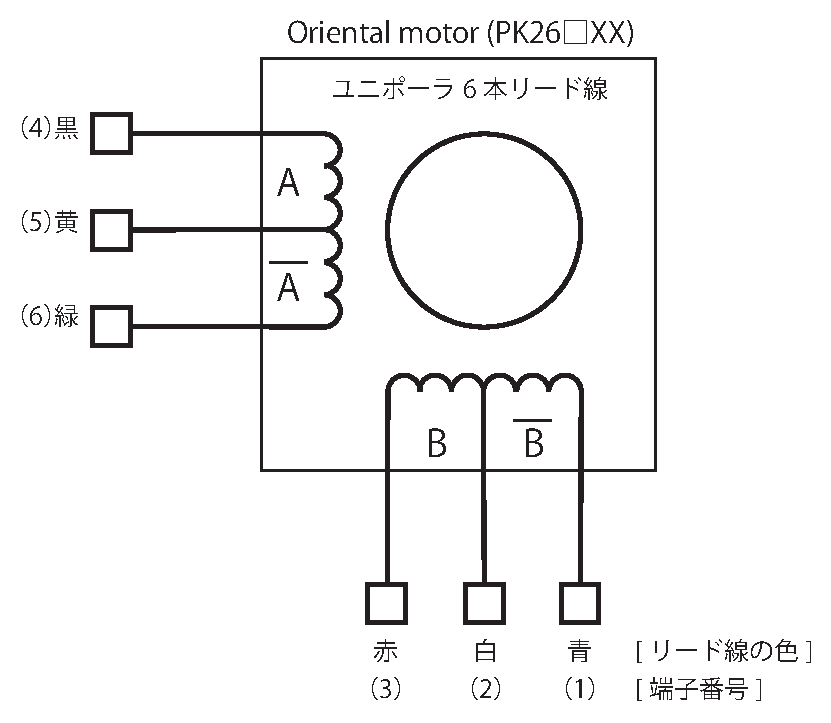
\includegraphics[keepaspectratio, scale=0.5, angle=0]
                            {figures/eps/stepper2.eps}
                            \caption{}
                            \label{fig:stepper2}
      \end{minipage}
    \end{minipage}
    \begin{minipage}{0.5\hsize}
      \begin{minipage}{0.90\hsize}
            \centering
            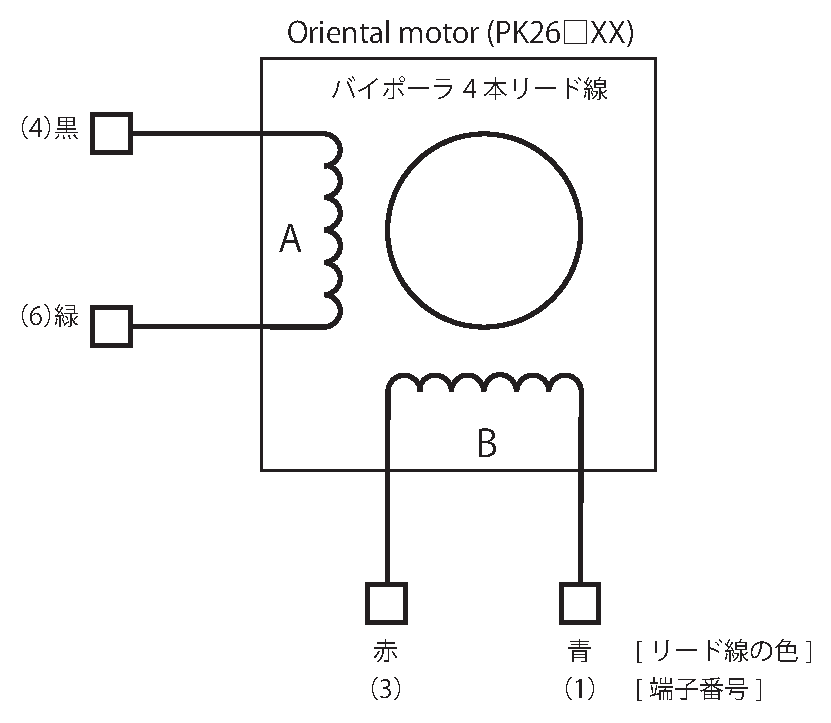
\includegraphics[keepaspectratio, scale=0.5, angle=0]
                            {stepper3.eps}
                            \caption{}
                            \label{fig:stepper3}
      \end{minipage}
    \end{minipage}
  \end{tabular}
\end{figure}%

\begin{minipage}{0.50\hsize}
      \centering
      \includegraphics[keepaspectratio, scale=0.45, angle=0]
                      {28BYJ-48.eps}
                      %\caption{}
                      \label{fig:stepper1}
\end{minipage}\\

\url{https://www.raspberrypi-spy.co.uk/2012/07/stepper-motor-control-in-python/}

\begin{lstlisting}[caption=Stepping Motor(Python),label=prog4]
# Import required libraries
import sys
import time
import RPi.GPIO as GPIO

# Use BCM GPIO references
# instead of physical pin numbers
GPIO.setmode(GPIO.BCM)

# Define GPIO signals to use
# Physical pins 11,15,16,18
# GPIO17,GPIO22,GPIO23,GPIO24
StepPins = [17,22,23,24]

# Set all pins as output
for pin in StepPins:
  print "Setup pins"
  GPIO.setup(pin,GPIO.OUT)
  GPIO.output(pin, False)

# Define advanced sequence
# as shown in manufacturers datasheet
Seq = [[1,0,0,1],[1,0,0,0],[1,1,0,0],[0,1,0,0],\
       [0,1,1,0],[0,0,1,0],[0,0,1,1],[0,0,0,1]]

StepCount = len(Seq)
StepDir = 1 # Set to 1 or 2 for clockwise
            # Set to -1 or -2 for anti-clockwise

# Read wait time from command line
if len(sys.argv)>1:
  WaitTime = int(sys.argv[1])/float(1000)
else:
  WaitTime = 10/float(1000)

# Initialise variables
StepCounter = 0

# Start main loop
while True:

  print StepCounter,
  print Seq[StepCounter]

  for pin in range(0, 4):
    xpin = StepPins[pin]
    if Seq[StepCounter][pin]!=0:
      print " Enable GPIO %i" %(xpin)
      GPIO.output(xpin, True)
    else:
      GPIO.output(xpin, False)

  StepCounter += StepDir

  # If we reach the end of the sequence
  # start again
  if (StepCounter>=StepCount):
    StepCounter = 0
  if (StepCounter<0):
    StepCounter = StepCount+StepDir

  # Wait before moving on
  time.sleep(WaitTime)
\end{lstlisting}%

%\subsection{Raspberry pi}

%\subsection{Arduino}



\chapter{アナログ入出力}

\section{可変抵抗器}

\subsection{電圧測定}

\subsection{トランジスタの特性測定}

\section{CdS(入力)}

\subsection{スイッチとしての利用}

\section{Strain gauge(入力)}

%\subsection{Raspberry pi}

%\subsection{Arduino}

\section{DC Motor(出力)}

%\subsection{Raspberry pi}

%\subsection{Arduino}

\chapter{スピーカ}

%\section{Raspberry pi}

%\section{Arduino}

\chapter{その他}

\section{Ir(赤外線送受信)}

LIRC(Linux Infrared Remote Control)を使って、

(1)家電機器のリモコンの信号を受信し、受信したIR信号を解析します

(2)解析したIR信号を、家電機器に送信して機器を操作します

\subsection{LIRCのインストール}

\begin{screen}\begin{verbatim}
sudo apt-get install lirc
\end{verbatim}\end{screen}

\subsubsection{/boot/config.txt}

50行目あたりを修正

赤外線受光器からの信号を受信するGPIOのピン番号をgpio\_in\_piに指定し、赤外線LEDへの出力に使うピンの番号をgpio\_out\_pinに指定します

\begin{screen}\begin{verbatim}
dtoverlay=lirc-rpi
dtparam=gpio_in_pin=26
dtparam=gpio_out_pin=27
\end{verbatim}\end{screen}

修正後は再起動します

\subsubsection{/etc/lirc/lirc\_options.conf}

\begin{screen}\begin{verbatim}
# devinput を default に
driver = devinput
↓
driver = default

# auto を /dev/lirc0 に
device = auto
↓
device = /dev/lirc0
\end{verbatim}\end{screen}

devinput.conf は削除する

\begin{screen}\begin{verbatim}
cd /etc/lirc/lirc.conf.d/
sudo rm -i devinput.conf
\end{verbatim}\end{screen}

\subsection{回路}

\subsection{IRデータの受信}

一旦、lircdを止めます

\begin{screen}\begin{verbatim}
sudo systemctl stop lircd
\end{verbatim}\end{screen}

以下コマンド実行

\begin{screen}\begin{verbatim}
mode2 -d /dev/lirc0 | tee ~/irdata.txt
\end{verbatim}\end{screen}

次のように、入力待ちの状態になる

\begin{screen}\begin{verbatim}
Trying device: /dev/lirc0
Using device: /dev/lirc0
\end{verbatim}\end{screen}

この状態でリモコンを受光器に向けて操作し、信号を受信させる

\begin{screen}\begin{verbatim}
Using driver default on device /dev/lirc0
space 16777215
pulse 3328
space 1576
pulse 469
space 359
pulse 477
space 354
pulse 473
space 1180
pulse 470
space 357
pulse 481
....
\end{verbatim}\end{screen}

ctrl+c で実行終了

保存したirdata.txtを編集します

一行目の、Using driver default on device /de/lirc0 を削除

2行目の、space 〜 も削除

以下pulseやspaceの文字を削除して、数値を羅列

適当な長さで改行(¥n)してよい

\begin{screen}\begin{verbatim}
3328 1576 469 359 477 354
473 1180 470 357 481
....
\end{verbatim}\end{screen}

機器のリモコンで、ONの時の信号のデータ、OFFの時の信号のデータを、それぞれ別のファイルに保存しておきます


\section{julius(音声認識)}

\url{https://www.raspberrypirulo.net/entry/julius}

\subsection{インストール準備}

\subsubsection{オーディオモジュールの優先順位}

usbオーディオアダプタ(snd\_usb\_audio)の優先順位を確認します。

内部オーディオデバイス(snd\_bcm2835)の優先順位が高くなっている場合は、優先順位を変更します。

下記のコマンドで現在の状態を確認できます。

\begin{screen}
\begin{verbatim}
$ cat /proc/asound/modules
  0 snd_bcm2835
  1 snd_usb_audio
\end{verbatim}
\end{screen}

/etc/modprobe.d/alsa-base.conf を新規作成して優先順位を変更できます

\begin{screen}
\begin{verbatim}
options snd slots=snd_usb_audio,snd_bcm2835
options snd_usb_audio index=0
options snd_bcm2835 index=1
\end{verbatim}
\end{screen}

再起動後、再度確認してUSB優先になってたらOk

\begin{screen}
\begin{verbatim}
$ cat /proc/asound/modules
  0 snd_usb_audio
  1 snd_bcm2835
\end{verbatim}
\end{screen}

\subsubsection{snd-pcm-ossモジュール}

juliusが使用するsnd-pcm-ossモジュールを起動時に毎回起動するように設定

\begin{screen}
\begin{verbatim}
$ sudo sh -c "echo snd-pcm-oss >> /etc/modules"
\end{verbatim}
\end{screen}

※注意事項

最新版のosの場合、snd-pcm-ossモジュールのロードでエラーになる場合があります。
"sudo modprobe snd-pcm-oss"コマンドを実行して、エラーになるかどうかを確認してください。
エラーになる場合は、"sudo apt-get install osspd-alsa"コマンドを実行して、osspd-alsaをインストールしてください。

\subsubsection{Juliusのインストール}

ファイルをダウンロードし、インストールを行います。
今回バージョンは4.4.2になります。(現在のカレントフォルダにファイルがダウンロードされます。)

\begin{screen}
\begin{verbatim}
$ mkdir ~/julius
$ cd ~/julius
$ wget https://ja.osdn.net/projects/julius/downloads/66547/julius-4.4.2.tar.gz
$ tar xvzf julius-4.4.2.tar.gz
$ cd ./julius-4.4.2
$ ./configure
$ make
$ sudo make install
\end{verbatim}
\end{screen}

何かエラーが発生する場合は、下記のモジュールをインストール後、再度実行してみます

\begin{screen}
\begin{verbatim}
$ sudo apt-get install build-essential zlib1g-dev libsdl2-dev libasound2-dev
\end{verbatim}
\end{screen}

ディクテーション実行キットを使う方法と、記述文法音声認識キットを使う方法の2つがありますので、それぞれ説明していきます。

\subsection{ディクテーション実行キットで音声認}

ディクテーションキットには、日本語のディクテーション(自動口述筆記)に必要な最小限のモデル
および Julius の実行バイナリが含まれています。

ですので、これだけでJulius を動かすことができ、使い方も簡単です。
処理速度、精度ともにあまりよくないですが、これだけで音声認識をすることができます(それなりに動きます)。

\subsubsection{ディクテーションキットの導入}

ホームディレクトリにdictationというフォルダ(フォルダ名は任意)を作って、その中にディクテーションキットをダウンロードし、解凍します。

\begin{screen}
\begin{verbatim}
$ mkdir ~/julius/dictation
$ cd ~/julius/dictation
$ wget https://osdn.net/projects/julius/downloads/66544/dictation-kit-v4.4.zip
$ unzip dictation-kit-v4.4.zip
\end{verbatim}
\end{screen}

\subsubsection{音声認識の動作確認}

下記コマンドを実行して、何か話すと話した言葉が表示されます。

\begin{screen}
\begin{verbatim}
$ cd ~/julius/dictation/dictation-kit-v4.5
$ julius -C main.jconf -C am-gmm.jconf -demo
\end{verbatim}
\end{screen}

\subsection{記述文法音声認識キットで音声認識}

記述文法音声認識は自分で辞書と文法ファイルを作成して、音声認識を行います。これにより、認識精度を上げることができ、処理速度も速くなります。

\subsubsection{記述文法音声認識キットの導入}

ホームディレクトリにdictというフォルダ(フォルダ名は任意)を作って、その中に記述文法音声認識キットをダウンロードし、解凍します。

\begin{screen}
\begin{verbatim}
$ mkdir ~/julius/dict
$ cd ~/julius/dict
$ wget https://github.com/julius-speech/grammar-kit/archive/v4.3.1.zip
$ unzip v4.3.1.zip
\end{verbatim}
\end{screen}

\subsubsection{辞書ファイルの作成}

はじめに簡単に辞書ファイルを作成する流れを説明します。

\begin{enumerate}
\item 日本語で読み仮名をふったファイルを作ります(tenki.yomi)
\item 読み仮名をローマ字に変換します(tenki.dic)
\item コンパイル出来る形式に編集します(tenki.voca)
\end{enumerate}

まず、音声認識したい単語を列挙して、日本語で読み仮名をふります。
単語間はタブ区切りで、最終行は改行が入らないようにします。
下記コマンドでtenki.yomiファイルを新規作成し、ファイルに単語を記載していきます。

\begin{screen}
\begin{verbatim}
  天気     てんき
  は     は
  晴れ     はれ
  曇り     くもり
  雨     あめ
  です     です
\end{verbatim}
\end{screen}

次に下記のコマンドを実行し、yomiファイルからdicファイルを生成します。このコマンドで日本語の読み仮名がローマ字になります。

\begin{screen}
  \begin{verbatim}
$ iconv -f utf8 -t eucjp ~/julius/dict/tenki.yomi | yomi2voca.pl | \
  iconv -f eucjp -t utf8 > ~/julius/dict/tenki.dic
\end{verbatim}
\end{screen}

生成されたtenki.dicを同じフォルダ内にコピーしてtenki.vocaファイルを作ります。

\begin{screen}
\begin{verbatim}
$ cp ~/julius/dict/tenki.dic ~/julius/dict/tenki.voca
\end{verbatim}
\end{screen}

tenki.vocaファイルを以下のように編集します。(タブ区切りはスペースに)

\begin{screen}
  \begin{verbatim}
  % TENKI
  天気   t e N k i
  % WA
  は   h a
  % TENKOU
  晴れ   h a r e
  曇り   k u m o r i
  雨   a m e
  % DESU
  です   d e s u
  % NS_B
  [s] silB
  % NS_E
  [/s] silE
\end{verbatim}
\end{screen}

\subsubsection{文法ファイルの作成}

新規ファイル(ファイル名:tenki.grammar)を生成し、下記のように記述します。

\begin{screen}
\begin{verbatim}
S : NS_B TENKI WA TENKOUDESU NS_E
  TENKOUDESU : TENKOU
  TENKOUDESU : TENKOU DESU
\end{verbatim}
\end{screen}

\begin{itemize}
\item TENKI ⇒ 上記の\%TENKIの単語を音声認識します。
\item WA ⇒ 上記の\%WAの単語を音声認識します。
\item TENKOUDESU ⇒ 上記の\%TENKOUもしくは\%TENKOU DESUの単語を音声認識します。
\item NS\_B ⇒ 文頭に挿入します。
\item NS\_E ⇒ 文末に挿入します。
\end{itemize}

\subsubsection{コンパイル}

辞書ファイル(tenki.voca)、文法ファイル(tenki.grammar)を使って、コンパイルします。

\begin{screen}
\begin{verbatim}
$ cd ~/julius/julius-4.4.2/gramtools/mkdfa
$ mkdfa.pl ~/julius/dict/tenki
\end{verbatim}
\end{screen}

成功するとtenki.dfa,dict,termファイルが生成されます。

\subsubsection{音声認識の動作確認}

\begin{screen}
\begin{verbatim}
$ julius -C ~/julius/dict/grammar-kit-4.3.1/hmm_mono.jconf -input mic \
            -gram ~/julius/dict/tenki -nostrip
\end{verbatim}
\end{screen}

これで文法として登録した言葉を優先的に認識してくれます。"天気は晴れです"、"天気は雨"等と話して、正しく認識されるか確認してください。

\section{OpenCV(画像入出力)}

\section{Webアプリ(tomcat)}

サーブレットコンテナとしてtomcatを使い、
そこで公したWebページから、
アプリケーションを動作させる方法について考察する

そのアプリケーションとして、ここではまずSerilaを通して通信をするもの、そして
GPIOにアクセスするもの、以上の2つの場合を考えることにする

\subsection{javaの開発環境をリモートで使う}

\subsection{Serial入出力(java)}

\subsection{tomcatからSerial通信}

\subsection{tomcatからGPIO}

\section{shutdownボタン}

\url{http://denshikousaku.net/put-shutdown-and-reboot-button-on-raspberry-pi}

\url{https://qiita.com/slses/items/e701c1cb6490751a6040}

BCM6がGNDに落ちたことを検出して、シャットダウン(あるいは再起動)させる

\subsubsection{シャットダウン発行の処理}

/home/pi/Documents/python/にshutdown.pyという名前で保存します

短押しで「再起動」、長押しで「終了」します(LEDでボタンの認識状態を確認できます)

\begin{lstlisting}[caption=/home/pi/Documents/python/shutdown.py,label=prog4]
#!/usr/bin/python
# coding:utf-8

import RPi.GPIO as GPIO
import time
import os

LED_PIN = 5
SW_PIN = 6

GPIO.setwarnings( False )
GPIO.setmode( GPIO.BCM )
GPIO.setup( SW_PIN, GPIO.IN, pull_up_down=GPIO.PUD_UP )
GPIO.setup( LED_PIN, GPIO.OUT )
GPIO.output( LED_PIN, GPIO.LOW)

button_previous = 1
button_current = 1
brojac = 0
flag_pressed = 0

try:
    GPIO.wait_for_edge( SW_PIN, GPIO.FALLING )

    while True:
        button_current = GPIO.input( SW_PIN )
        flag_pressed = button_previous + button_current

        if ( not(flag_pressed) ):
            brojac += 1
        else:
            brojac = 0

        if( button_current and (not button_previous) ):
            GPIO.output( LED_PIN, GPIO.HIGH )
            os.system( "sudo shutdown -r now" )
            break
        if( (not flag_pressed) and brojac >= 100 ):
            GPIO.output( LED_PIN, GPIO.HIGH )
            os.system( "sudo shutdown -h now" )
            break

        button_previous = button_current
        time.sleep( 0.03 )

except KeyboardInterrupt:
    pass

finally:
    GPIO.cleanup()
\end{lstlisting}%

実行権限を付与

\begin{screen}
\begin{verbatim}
$ chmod +x shutdown.py
\end{verbatim}
\end{screen}

動作確認をします

\begin{screen}
\begin{verbatim}
$ ./shutdown.py &
\end{verbatim}
\end{screen}

\subsubsection{サービスファイルの作成}

/usr/lib/systemd/system/にshutdownbuttond.serviceという名前で保存

\begin{lstlisting}[caption=/usr/lib/systemd/system/shutdownbuttond.service,label=prog4]
[Unit]
Description=Shutdown Daemon

[Service]
ExecStart = /home/pi/Documents/python/shutdownd.py
Restart=always
Type=simple

[Install]
WantedBy=multi-user.target
\end{lstlisting}%

\subsubsection{サービスの有効化}

以下で有効化します(パスワードが要求されます)

\begin{screen}
\begin{verbatim}
$ systemctl enable shutdownbuttond.service
\end{verbatim}
\end{screen}

※注意事項:自動起動を無効化する際には、enableの部分をdisableに指定します

デーモンの再起動

\begin{screen}
\begin{verbatim}
$ sudo systemctl daemon-reload
\end{verbatim}
\end{screen}

サービスが有効になっているかどうかを確認

\begin{screen}
\begin{verbatim}
$ systemctl status shutdownbuttond.service
\end{verbatim}
\end{screen}

ここで、
(/usr/lib/systemd/system/shutdownbuttond.service; enabled)、
active (running)
となっていたらOk(再起動でactiveになる)

\begin{screen}
\begin{verbatim}
$ systemctl -t service
\end{verbatim}
\end{screen}

として全てのサービスを表示させることもできる

※注意事項

プログラムや設定などを誤ると、「起動直後に再起動を繰り返す!」
ことにもなりかねず、注意深く作業することが必要です

なお、
BCM3をGNDに落とすと、シャットダウン後に再起動させることもできるようです

\end{comment}

\chapter{おわりに}
\newpage
%
\section*{謝辞}
\addcontentsline{toc}{chapter}{謝辞}
%
\begin{thebibliography}{99}
  \bibitem{1}
\end{thebibliography}
%
% END DOCUMENT
\end{document}
%
